\section{Introduction}

The previous chapter characterised an open innovation partnership as a temporary organisation formed to facilitate the transfer of knowledge and achieve a specific innovation outcome. It went on to explain how social network analysis could be used to evaluate knowledge sharing practices in open innovation partnerships. Four propositions around the micro-structure of tacit knowledge networks were presented. This chapter considers the social forces that may influence how tacit knowing is applied in open innovation partnerships. \medskip

The extent to which structure inhibits or encourages agency in open innovation has not received much attention in the literature so far. Structure refers to the patterned arrangements that influence or limit the choices and opportunities available to individuals \citep{bandura1999social}. Human agency is about the capacity of individuals to act autonomously and make their own free choices \citep{giddens1984constitution,emirbayer1994network}. \medskip

In the case of open innovation, knowledge networks, organisational structures, rules and procedures may be considered examples of structure. The embryonic structure of knowledge networks may constrain agency. Participants are thrown together to form a temporary organisation that requires swift trust to function \citep{meyerson1996swift}. As time goes on participants will attempt to self-organise into groups of like-minded people. Agency is vital because it lies at the heart of tacit knowledge exchange and too much structure may inhibit participants' willingness to share tacit knowledge or contribute ideas \citep{lam2000tacit}. Conversely, too little structure can make goals less clear, leading to unsatisfactory open innovation outcomes. Finding the right balance between structure and agency is considered essential for successful open innovation \citep{davis2010agency}. \medskip

This chapter develops the theoretical framework used in this study to assess tacit knowledge behaviour in three open innovation partnerships. It reviews the structure versus agency debate before delving into theories of motivation, trust, and power. This study considers motivation, trust, and power to be key factors influencing tacit knowledge sharing behaviour. Key theoretical concepts are used to formulate additional propositions about tacit knowledge sharing in terms of motivation, trust, and power. 

\section{The structure versus agency debate}

The structure versus agency debate addresses a fundamental question: do social structures determine how individuals act or are social structures the product of individual action? There is a growing consensus that structure and agency are complementary. What remains a bone of contention, however, is how these complement each other \citep{tan2011understanding}. Much of the current debate centres around the concept of structure. \medskip

According to \citet{giddens1984constitution}, structure is not something external to the individual. He sees structure as patterns of practices. As practices change, so does structure, and vice-versa. \citet{giddens1984constitution} uses the term \enquote{duality of structure} to describe structure as both a medium and an outcome. \citet{archer1995realist} questions the inseparability of structure and agency. She argues that structure always precedes agency and that both operate on different timescales. At any particular moment, existing structures constrain and enable agents \citep{emirbayer1998agency}. Their interactions have both intended and unintended consequences that result in the reproduction or transformation of the initial structure. The reproduced or transformed structure provides context for future actions. Because the initial structure was itself a result of structural elaboration by prior agents, \citet{archer1998critical} argues that it is impossible to unpick them analytically. \medskip

The emerging critical realist perspective argues that individual action is influenced not just by the causal powers of social structures, but also by other interacting causal powers, including those of the individual concerned \citep{elder2008searching,elder2010causal,sorrell2018explaining}. Individual actions contribute to the reinforcement or transformation of the social structure concerned. In other words, both individuals and social structures have distinctive causal powers that interact to determine social events \citep{loyal2001agency}. Figure \ref{fig:agency_structure} illustrates how need-based actions are tempered by causal powers at both the individual and structural level \citep{loyal2001agency}. Agency is not a simple matter of having free choice. Instead, it involves making choices that balance individual need dispositions with internalised social norms and social reality \citep{loyal2001agency}. For instance, a partner's appropriability regime can impact inter-organisational knowledge sharing in both positive and negative ways. It may either inhibit knowledge sharing or facilitate knowledge sharing through clearly defined rules of engagement \citep{dahlander2010open,laursen2014paradox,llanes2018competitive}. \medskip

\begin{figure}[h!]
    \centering
    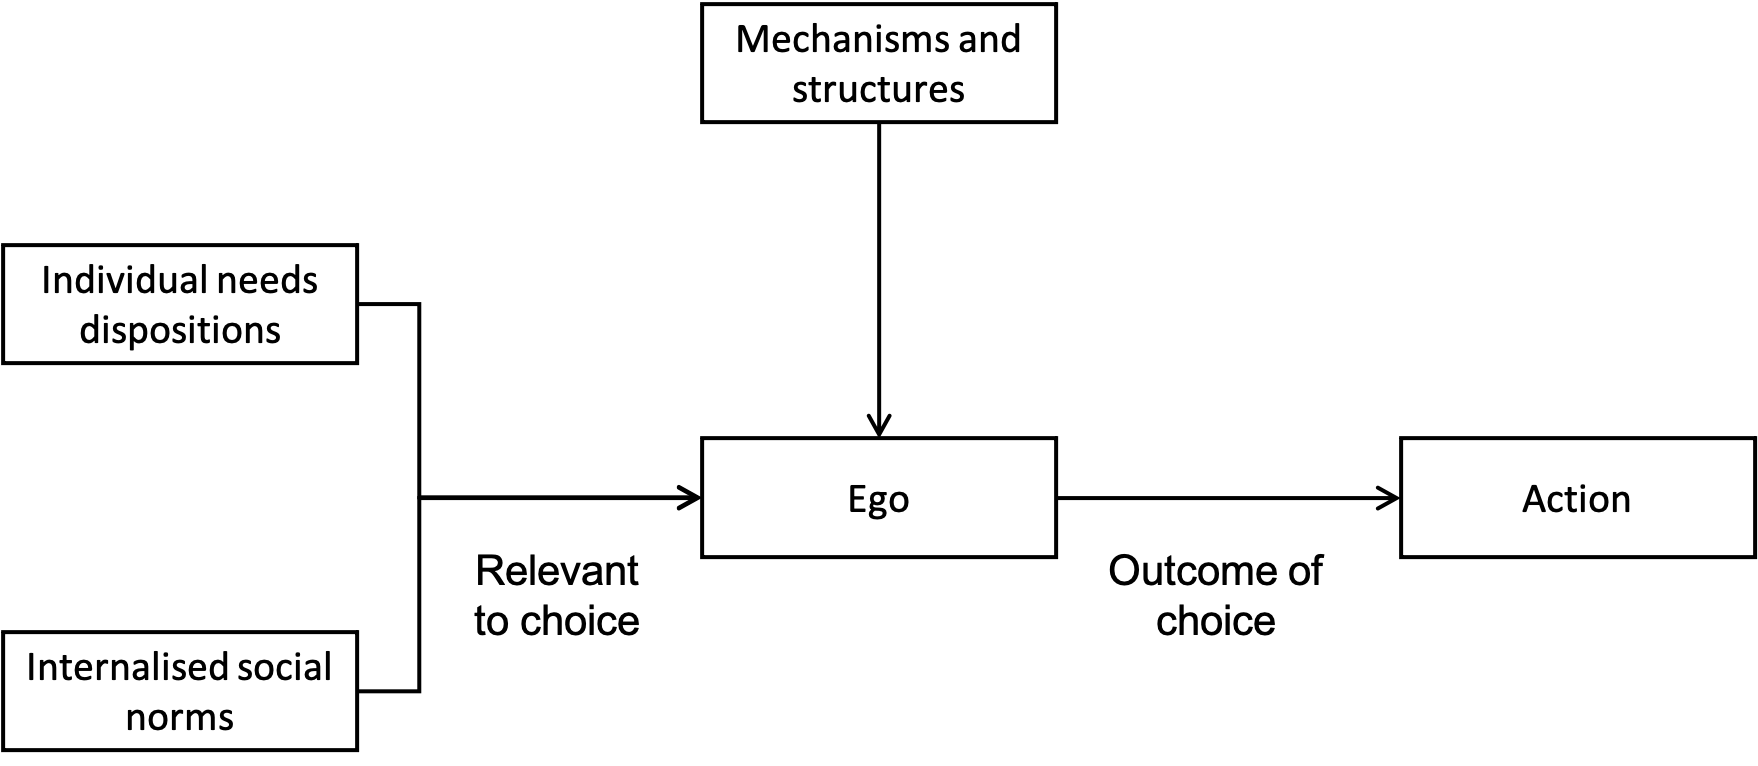
\includegraphics[width=0.9\textwidth]{Images/agency_structure_loyal.png}
    \caption[Critical realist perspective of agency versus structure]{Critical realist perspective of agency versus structure. Agency is about making choices to satisfy innate needs. These choices may be tempered by internalised social norms and social reality more broadly \citep{loyal2001agency}.}
    \label{fig:agency_structure}
\end{figure}

When considering the structure versus agency debate in open innovation, it is reasonable to assume that structures in each partner organisation do influence how individual participants interact across organisational boundaries \citep{llanes2018competitive}. One may argue that it is the actions of individual participants from each partner organisation that determine the functional structure of an open innovation partnership. In that sense, an open innovation partnership is both dynamic and emergent. Hence, \bigskip

\begin{tcolorbox}
\textit{\textbf{Proposition 3a:} Formal structures inhibit tacit knowledge exchange in open innovation partnerships (Research Question 3).}
\end{tcolorbox}

\section{Motivation}

A large part of agency is about humans striving to satisfy innate needs \citep{deci2001need}. The quest to satisfy such needs is what motivates people to act \citep{bandura1989human}. Motivation is a theoretical construct used to explain individual behaviour. More specifically, a motive is what prompts a person to act in a specific way or develop an inclination towards a particular behaviour \citep{pardee1990motivation}. \medskip

Motivation is the  driving force behind creativity and innovation  \citep{amabile1988model,hennessey2010creativity}. Open innovation is less likely to succeed without highly motivated agents, i.e. individuals who are willing to take risks and make the effort to learn from, or share their know-how or expertise with, others \citep{nonaka1994dynamic,leonard1998role,bock2005behavioral}. 

\subsection{Quest for self-efficacy}

Humans exercise agency through self-belief in their ability to manage prospective situations, also referred to as their sense of personal self-efficacy \citep{white1959motivation, bandura1994self}. The quest for self-efficacy drives individual learning, much of which is achieved by observing how others behave or act \citep{bandura1986social}. By observing others, an individual can assess the outcomes of different patterns of behaviour, which then serves as a guide for future action, thereby helping them develop a stronger sense of self-efficacy \citep{bandura1977self,bandura1999social}. 

\subsection{Level of self-determination}

Self-determination theory suggests that humans are innately driven to seek out competence (personal self-efficacy), autonomy (rights to agency) and social relatedness \citep{ryan2000self}. The theory distinguishes between controlled and autonomous motivation. Being controlled involves acting under some sense of social pressure (subjective norm). Autonomy involves acting with a sense of volition and having the experience of choice. Intrinsic motivation, driven by an individual's interest or pleasure in the activity itself, is mostly autonomous. Less engaging activities require extrinsic motivation, where people's actions depend on the perceived contingency between behaviour and the desire for implicit approval or tangible rewards \citep{gagne2005self}. Extrinsic motivation can vary in the degree to which it is autonomous or controlled. Externally regulated behaviour is a form of controlled motivation. Regulation that has been taken in by a person but not accepted as their own is said to be \enquote{introjected} and is a form of internalised extrinsic motivation. With \enquote{identified regulation}, people feel a greater sense of autonomy because their behaviour aligns with their personal beliefs \citep{gagne2005self}. \medskip

Past studies show that autonomous motivation facilitates effective performance and well-being, whereas controlled motivation can detract from those outcomes, especially if the task requires creativity, cognitive flexibility, or deep processing of information \citep{gagne2005self}. \citet{gagne2009model} presents a process model of knowledge-sharing motivation based on the theory of planned behaviour and self-determination theory. The model assumes that autonomous motivation predicts knowledge sharing intention, which in turn predicts knowledge-sharing behaviour. The more internalised the individual's motivation to share knowledge, the more likely knowledge sharing will result \citep{gagne2009model,witherspoon2013antecedents}. \medskip

As long as knowledge sharing is voluntary, sharing parties tend to perceive it as intrinsically satisfying because it is self-determined and enhances their sense of self-efficacy \citep{lam2010knowledge,dumbach2014establishing}.  Tacit knowledge is less likely to be shared freely in organisations that rely heavily on incentive schemes to motivate employees. Since tacit knowledge sharing is a social act, it also satisfies an individual's need for relatedness \citep{llopis2016understanding}. People who are autonomously motivated are thus more likely to build their know-how or expertise compared to those inclined towards controlled motivation.

\subsection{Intention to seek or share knowledge}

The theory of planned behaviour claims actions and behaviours reliably follow intentions. Intentions capture the normative and conditional elements that influence a particular behaviour \citep{ajzen1985intentions}. The theory of planned behaviour posits three conceptually independent determinants of intention: First is \textit{attitude} toward the behaviour, which refers to the degree to which an individual has a favourable or unfavourable disposition towards the behaviour in question. Second is \textit{subjective norm} that refers to the perceived social pressure to perform or not to perform the behaviour, which can vary according to how internalised the norm is, the strength of the desire to overcome opposition to that behaviour and the amount of effort that is required to conform to the norm \citep{loyal2001agency}. Third is the \textit{degree of perceived self-efficacy}, which, as stated earlier, refers to how people rate their ability to manage prospective situations \citep{bandura1982self,ajzen1991theory}. \medskip

The theory of planned behaviour implies an individual's motivation to seek out or share tacit knowledge is not only dependent on their perceived self-efficacy but is also dependent on their attitudes and subjective norms. Individuals will be more inclined to seek out or share tacit knowledge if this is perceived as normal or acceptable behaviour and does not require too much effort \citep{gagne2009model,chen2012behavioral}. \bigskip

\begin{tcolorbox}
\textit{\textbf{Proposition 3b:} Innate needs and subjective norms moderate individual willingness to seek out or share tacit knowledge (Research Question 3).}
\end{tcolorbox}

\section{Trust}

Trust is \enquote{the willingness of a party to be vulnerable to the actions of another party based on the expectation that the other will perform a particular action important to the trustor, irrespective of the ability to monitor or control that other part} \citep{mayer1995integrative}. 
Trust is an enabler of human agency as it facilitates human action \citep{muller2008living,mcevily2011measuring}. Trust also limits opportunistic behaviour, reduces uncertainty, builds commitment, facilitates cooperation, and creates a safe environment in which to resolve issues \citep{nonaka1994dynamic,panteli2005trust,rasmussen2007work}. People are inclined to hoard their tacit knowledge to maintain some form of advantage and are unlikely to disclose such knowledge if this will make them feel more vulnerable  \citep{levin2004strength,kankanhalli2005contributing,riege2005three,lin2007share,milne2007motivation,alsharo2017virtual}. 

\subsection{Cognition- and affect\hyp{}based trust}

Trust is cognition-based insofar as \enquote{we choose whom we will trust in which respects and under what circumstances, and we base the choice on what we take to be \enquote{good reasons}, constituting evidence of trustworthiness} \citep{lewis1985trust}. Innovation often requires people to take risks, and cognition\hyp{}based trust plays a key role in deciding whether to take a leap of faith or not \citep{mcevily2011measuring}. Affect-based trust consists of the emotional bonds between individuals and relates to care and concern for the welfare of another \citep{mcallister1995affect}. \medskip

Past studies reveal that affect\hyp{}based trust has a significantly greater effect on willingness to \textit{share} tacit knowledge, whereas cognition-based trust plays a greater role in willingness to \textit{use} tacit knowledge \citep{levin2004strength,holste2010trust,ding2015research}. 

\subsection{Reciprocal nature of trust}

Reciprocity is an indicator of trust in social networks. Reciprocity is a key concept in social exchange and game theory and reflects a human tendency to return helpful or harmful acts in kind \citep{nowak2005evolution}. According to social exchange theory, individuals act to maximise the potential of economic and social returns \citep{homans1961social,blau1964exchange}. A person does another a favour with a general expectation of some future non-binding return. Trust is more likely to develop between partners when exchange occurs without explicit negotiations or binding agreements. Under such conditions, the risk and uncertainty of exchange provide the opportunity for partners to demonstrate their trustworthiness \citep{molm2000risk}. Inadequate reinforcement or asymmetry in economic or social returns may result in the breakdown of trust \citep{homans1961social}. \medskip

In game theory, the \enquote{prisoner’s dilemma} is a game that explores the tension between individual self-interest and collective cooperation \citep{richards2001reciprocity}. Individuals or groups are assumed to be primarily motivated by self-interest. Modelling of the \enquote{prisoner's dilemma} shows that people can maximise their payoff through cooperative action based on simple reciprocity or \enquote{tit-for-tat} behaviour \citep{axelrod1980effective,axelrod1981evolution}. Tit-for-tat involves cooperating with your partner on the first round, then adjusting your behaviour to match your partner’s in subsequent rounds. If your partner cooperates in a reciprocal manner, you continue to cooperate. However, should they defect, you respond in kind by retaliating immediately against them. The assumption is that people who start out with good intentions (e.g. by being nice, generous, or forgiving) are more likely to be cooperative \citep{blais1987epistemic,richards2001reciprocity,fulmer2013trust}. This implies people will not be inclined to share tacit knowledge unless they see some personal advantage to do so \citep{yang2006knowledge,singh2019territoriality}. 

\subsection{Network closure}

Network closure is another indicator of trust in social networks. It refers to the tendency for humans to form social groups and reflects the extent to which everyone knows everyone else in a network \citep{coleman1990foundations}. Network or triadic closure can be summarised as \enquote{a friend of a friend is a friend} and refers to the formation of triangles in a social network. Triangles represent archetypal social groups \citep{robins2015doing}. Network closure creates social conditions that build mutual trust. Promises made within a group can usually be trusted because the consequences of breaking a promise would be dire. In a network of three people (A, B and C), A can monitor B directly but also indirectly through C. Anyone who breaks trust in a small social group would soon find themselves ostracised. What builds trust in small social groups is the expectation that people will behave in prescribed ways to protect their reputation \citep{burt2005brokerage}. 

\subsection{Swift trust}

Trust usually develops gradually over time through observations of past behaviour \citep{mayer1995integrative}. Achievement of trust at one level enables the development of trust at the next level and so on \citep{robert2009individual}. Swift trust is a presumptive form of trust that may explain trusting behaviour exhibited by members of temporary organisations\footnote{A temporary organisation is a \enquote{a temporally bounded group of interdependent organisational actors, formed to complete a complex task} \citep{burke2016temporary}, which is an apt description of an open innovation partnership}. Team members \enquote{suspend doubt} about the dependability of unknown others to accomplish a task \citep{germain2014role}. Influenced by their disposition towards trust, team members use \enquote{category-based information processing} to form an initial swift trust judgement by mentally placing others into a specific trust category. Adjustments are made to trust beliefs according to fulfilled or unfulfilled expectations \citep{meyerson1996swift,robert2009individual}. \medskip

People tend to respond favourably to swift trust, which contributes to positive working relationships. High-trusting temporary organisations are more likely to exhibit high-performance \citep{ashleigh2007trust}. Swift trust is vital in temporary organisations because it substitutes the traditional mechanisms of control and coordination found in established organisational hierarchies \citep{kasper2001communicating}. \bigskip

\begin{tcolorbox}
\textit{\textbf{Proposition 4a:} Reciprocity and closure in tacit knowledge exchange networks indicate high levels of trust in   open innovation partnerships (Research Question 4).}
\end{tcolorbox}

\section{Power}

As noted in the previous chapters (Sections 1.3.3 and 2.5), two contrasting views of power dominate the literature: \enquote{power as domination}, otherwise referred to as \enquote{power-over}, and \enquote{power as empowerment}, also known as \enquote{power-to} \citep{haugaard2012rethinking}. This section explores how both forms of power may moderates tacit knowledge sharing in terms of structuration theory, power-dependence theory, and self-determination theory. 

\subsection{Power of tacit knowledge}

According to \citeauthor{giddens1984constitution}'s \citeyearpar{giddens1984constitution} structuration theory, agents derive their power from existing social structures that enable them to exercise power over others or affords them power to intervene in specific social situations. \citet{giddens1984constitution} considers \enquote{power-over} to be a subset of \enquote{power to}. For him, \enquote{power-to} is a transformative capacity that can change practices or structures. He sees \enquote{power-to} as something that resides in the \enquote{knowledgeability} of actors who know exactly what to do in different social contexts (what \citet{polanyi1966logic} refers to as \enquote{tacit knowing}). This aligns with the thinking of \citet{foucault1980power}, who argues power is knowledge and is inherent in all social relations where people negotiate meaning in terms of accepted forms of knowledge, scientific understanding, and truth \citep{diamond1988foucault}. Tacit knowledge is a tremendous source of personal power, especially for those lower down the organisational hierarchy \citep{bordum2002tacit,gourlay2002tacit}. Attempts by organisations to codify the tacit knowledge embodied in their employees may be seen as a way of neutralising this power \citep{schultze2004knowing,singh2019territoriality}. By applying their tacit knowledge, people are exercising \enquote{power-to} bring about change \citep{schultze2004knowing,lam2014tacit}. This implies tacit knowledge lies at the very heart of the structure versus agency debate \citep{lam2000tacit,lam2014tacit}. 

\subsection{Power as a relational construct}

Both power-over and power-to treat power as a relational construct, where the distribution of power reflects the structure of exchange opportunities \citep{blau1964exchange,reagans2008knowledge,bonacich2009structural}. The power of one actor over another reflects the dependence of the second on the first for a valued resource \citep{emerson1962power}. Preferential attachment theory suggests actors prefer to attach to well-connected actors over poorly-connected actors \citep{barabasi1999emergence}. The consequence of this is that more central actors in a knowledge exchange network will acquire knowledge at a faster rate than others. This has implications for power-dependence relations. More central actors are able to exert much more influence because they have greater access to diverse knowledge and are able to dictate agendas \citep{bonacich1987power,foucault1980power}. \medskip

Power imbalances may lead those feeling disempowered or powerless to engage in cost-reduction or balancing operations \citep{emerson1962power}. Cost-reduction is a process in which a person adjusts his or her personal values to accommodate the demands of a powerful other. The less powerful person simply acquiesces to the more powerful other. Such behaviour does not alter the balance of power. Balancing operations, on the other hand, aim to shift the balance of power. For example, tensions generated by power inequality can result in network extension where power-disadvantaged actors may seek out new social connections to reduce their dependence on a given actor for valued resources \citep{cook2013social}. Other ways to balance power include motivational withdrawal or deference \citep{emerson1962power}. Balancing operations illustrate how the distinctive causal powers of both individuals and social structures interact to determine social outcomes \citep{loyal2001agency}. \medskip

\enquote{Power-to} can also be treated as a relational construct. Powerful actors can empower others through power sharing or delegating authority. Since powerful actors control who they share power with or delegate authority to, this may be perceived as a limited form of empowerment \citep{conger1988empowerment}. Power-over others has been identified as barriers to knowledge sharing \citep{riege2005three,suppiah2011organisational}. People in authority often serve as gatekeepers of knowledge to preserve or enhance their status \citep{cross2001beyond}. Actors who do not award status to more powerful actors are likely to withhold their tacit knowledge from them \citep{cabrera2006determinants}. However, actors may be more willing to seek out tacit knowledge from more central actors whose power stems from deference relating to their expertise. Alternatively, actors more likely to share tacit knowledge with others at a similar level of power as them \citep{cabrera2006determinants}. 

\subsection{Power as a motivational construct}

Earlier it was stated that individuals are motivated to achieve greater self-efficacy to better manage prospective situations they may find themselves in. The quest for self-efficacy drives individual learning, much of which is achieved by observing how others behave or act. Individuals empower themselves by accumulating tacit knowledge. The know-how and expertise helps them cope with the physical and social demands of the environment. Individuals who share their hard-earned know-how or expertise are empowering others. Any strategy that undermines the self-efficacy of organisational members will increase their feelings of powerlessness. This speaks directly to the \enquote{agency versus structure} debate, i.e. power-to promotes human agency whereas structure is about exercising power-over others.

\subsection{Relationship between trust and power}

In a power-dependence relation, a powerful actor can reasonably expect the less powerful other to place a high value on their exchange relationship because the less powerful person does not have many options to access this resource elsewhere \citep{emerson1962power}. \citet{schilke2015power} find that power-disadvantaged actors tend to be more trusting than powerful actors. They suggest with increasing dependence, power-disadvantaged actors invest more cognitive resources in processing trust-related information that becomes available in an exchange than more powerful actors. Power-disadvantaged actors are likely to see the more powerful other as trustworthy to avoid anxiety stemming from their feelings of dependence. \citet{schilke2015power} suggest hope and perceived benevolence feature strongly in the trust decisions of power-disadvantaged. \medskip

Tacit knowledge is a tremendous source of personal power and deference. Resisting the formalisation of tacit knowledge can help maintain personal power \citep{schultze2004knowing}. While a power-disadvantaged actor might be less inclined to share their tacit knowledge with a more powerful other, they may end up doing so anyway to reduce anxiety. A more powerful actor may be less inclined to trust others with their tacit knowledge \citep{schilke2015power}. Hence, \bigskip

\begin{tcolorbox}
\textit{\textbf{Proposition 4b:} Who people choose to empower with their know-how depends on how much they trust the receiver to use their know-how in mutually beneficial ways (Research Question 4).} 
\end{tcolorbox}

\section{Summary}

The main argument of this chapter is that the quest for tacit knowledge drives agency. Agents acquire tacit knowledge to not only satisfy an innate need for competence, but also to gain sufficient power to maintain or enhance their autonomy and to influence agendas and enact change. This has implications in terms of structure versus agency. Two key assumptions guide our thinking going forward: First, agency lies at the heart of tacit knowledge sharing. Second, innovation depends on the application of know-how in new or different contexts. These two assumptions suggest that informal structure is an essential feature in any open innovation partnership. We can describe this informal structure as an intentional community of practice. One can argue that successful open innovation depends on the emergence of informal structure and how well this operates as an intentional community of practice. \medskip

Effective open innovation structures are those than recognise people are driven by a need for competence. Because tacit knowledge is a source of personal power, individuals are going to be very selective in who they choose to share their tacit knowledge with. They are unlikely to surrender their hard-earned tacit knowledge if the costs of doing so outweigh the benefits. Individuals are less likely to reveal their tacit knowledge to those they do not trust or those who have power over them. With respect to open innovation, formal structures and prevailing culture in each partner organisation are likely to influence how individual participants interact across organisational boundaries. Given the important role of tacit knowledge in innovation, open innovation partnerships must be structured in ways that promote personal agency. Participants need to be able to choose who they share their tacit knowledge with. They are unlikely to share their tacit knowledge with others if power-relations are imbalanced. Participants need to work hard and building and maintaining trust, not only at an interpersonal level, but at the organisational level as well. Failure to do so will limit the flow of tacit knowledge. \medskip

How well open innovation partnerships function in practice is determined not so much by formal structures and prevailing cultures, but by the actions of individual participants. One may argue open innovation success depends on the willingness of participants to share or seek out tacit knowledge. This willingness is moderated by personal levels of autonomous motivation, disposition to trust, and power-relations in different social contexts. A better understanding of how people are motivated to share their know-how may contribute to more effective knowledge management practices in open innovation.\medskip

The next chapter explains the methodology used to assess how motivation, trust, and power shape tacit knowledge sharing ties in open innovation partnerships. It includes justifications for embracing a critical realist worldview and need for a case-based mixed-method research design.